\documentclass[12pt,compress,ngerman,utf8]{beamer}
\usepackage[ngerman]{babel}
\usepackage{multicol}
\usepackage{animate}
\usepackage[protrusion=true,expansion=true]{microtype}

\DeclareSymbolFont{extraup}{U}{zavm}{m}{n}
\DeclareMathSymbol{\varheart}{\mathalpha}{extraup}{86}
\DeclareMathSymbol{\vardiamond}{\mathalpha}{extraup}{87}

\title{Matheschülerzirkel Augsburg}
\author{ingo.blechschmidt@math.uni-augsburg.de}
\date{Tübinger Linuxtag am 11. Juni 2016}

\usetheme{Warsaw}

\useinnertheme{rectangles}

\usecolortheme{seahorse}
\definecolor{mypurple}{RGB}{150,0,255}
\setbeamercolor{structure}{fg=mypurple}

\usefonttheme{serif}
\usepackage[T1]{fontenc}
\usepackage{libertine}

\setbeamertemplate{navigation symbols}{}
\setbeamertemplate{headline}{}
\setbeamertemplate{frametitle}[default][colsep=-2bp,rounded=false,shadow=false,center]

\renewcommand*\insertshorttitle{Matheschülerzirkel Augsburg}

\newcommand{\hil}[1]{{\usebeamercolor[fg]{item}{\textbf{#1}}}}

\newcommand{\imgslide}[1]{{\usebackgroundtemplate{\includegraphics[height=\paperheight]{#1}}\begin{frame}[plain]\end{frame}}}
\newcommand{\imgslidetrans}[1]{{\usebackgroundtemplate{\includegraphics[height=\paperheight]{#1}}\begin{frame}[plain]\transduration{5}\transfade[duration=0.3]\end{frame}}}
\begin{document}

% http://www.fussball-institut.de/wp-content/uploads/2014/10/Fussball.jpg
\imgslide{images/fussball}

% http://www.voofoostudios.com/wp-content/uploads/2014/05/Williams_PS_011.jpg
\imgslide{images/schach}

% https://upload.wikimedia.org/wikipedia/commons/b/b9/Hopf_Fibration.png
\imgslide{images/mathe}

{
  \usebackgroundtemplate{
\includegraphics[height=\paperheight,width=\paperwidth]{images/plakat-hintergrund}}
  \begin{frame}[plain]\centering
    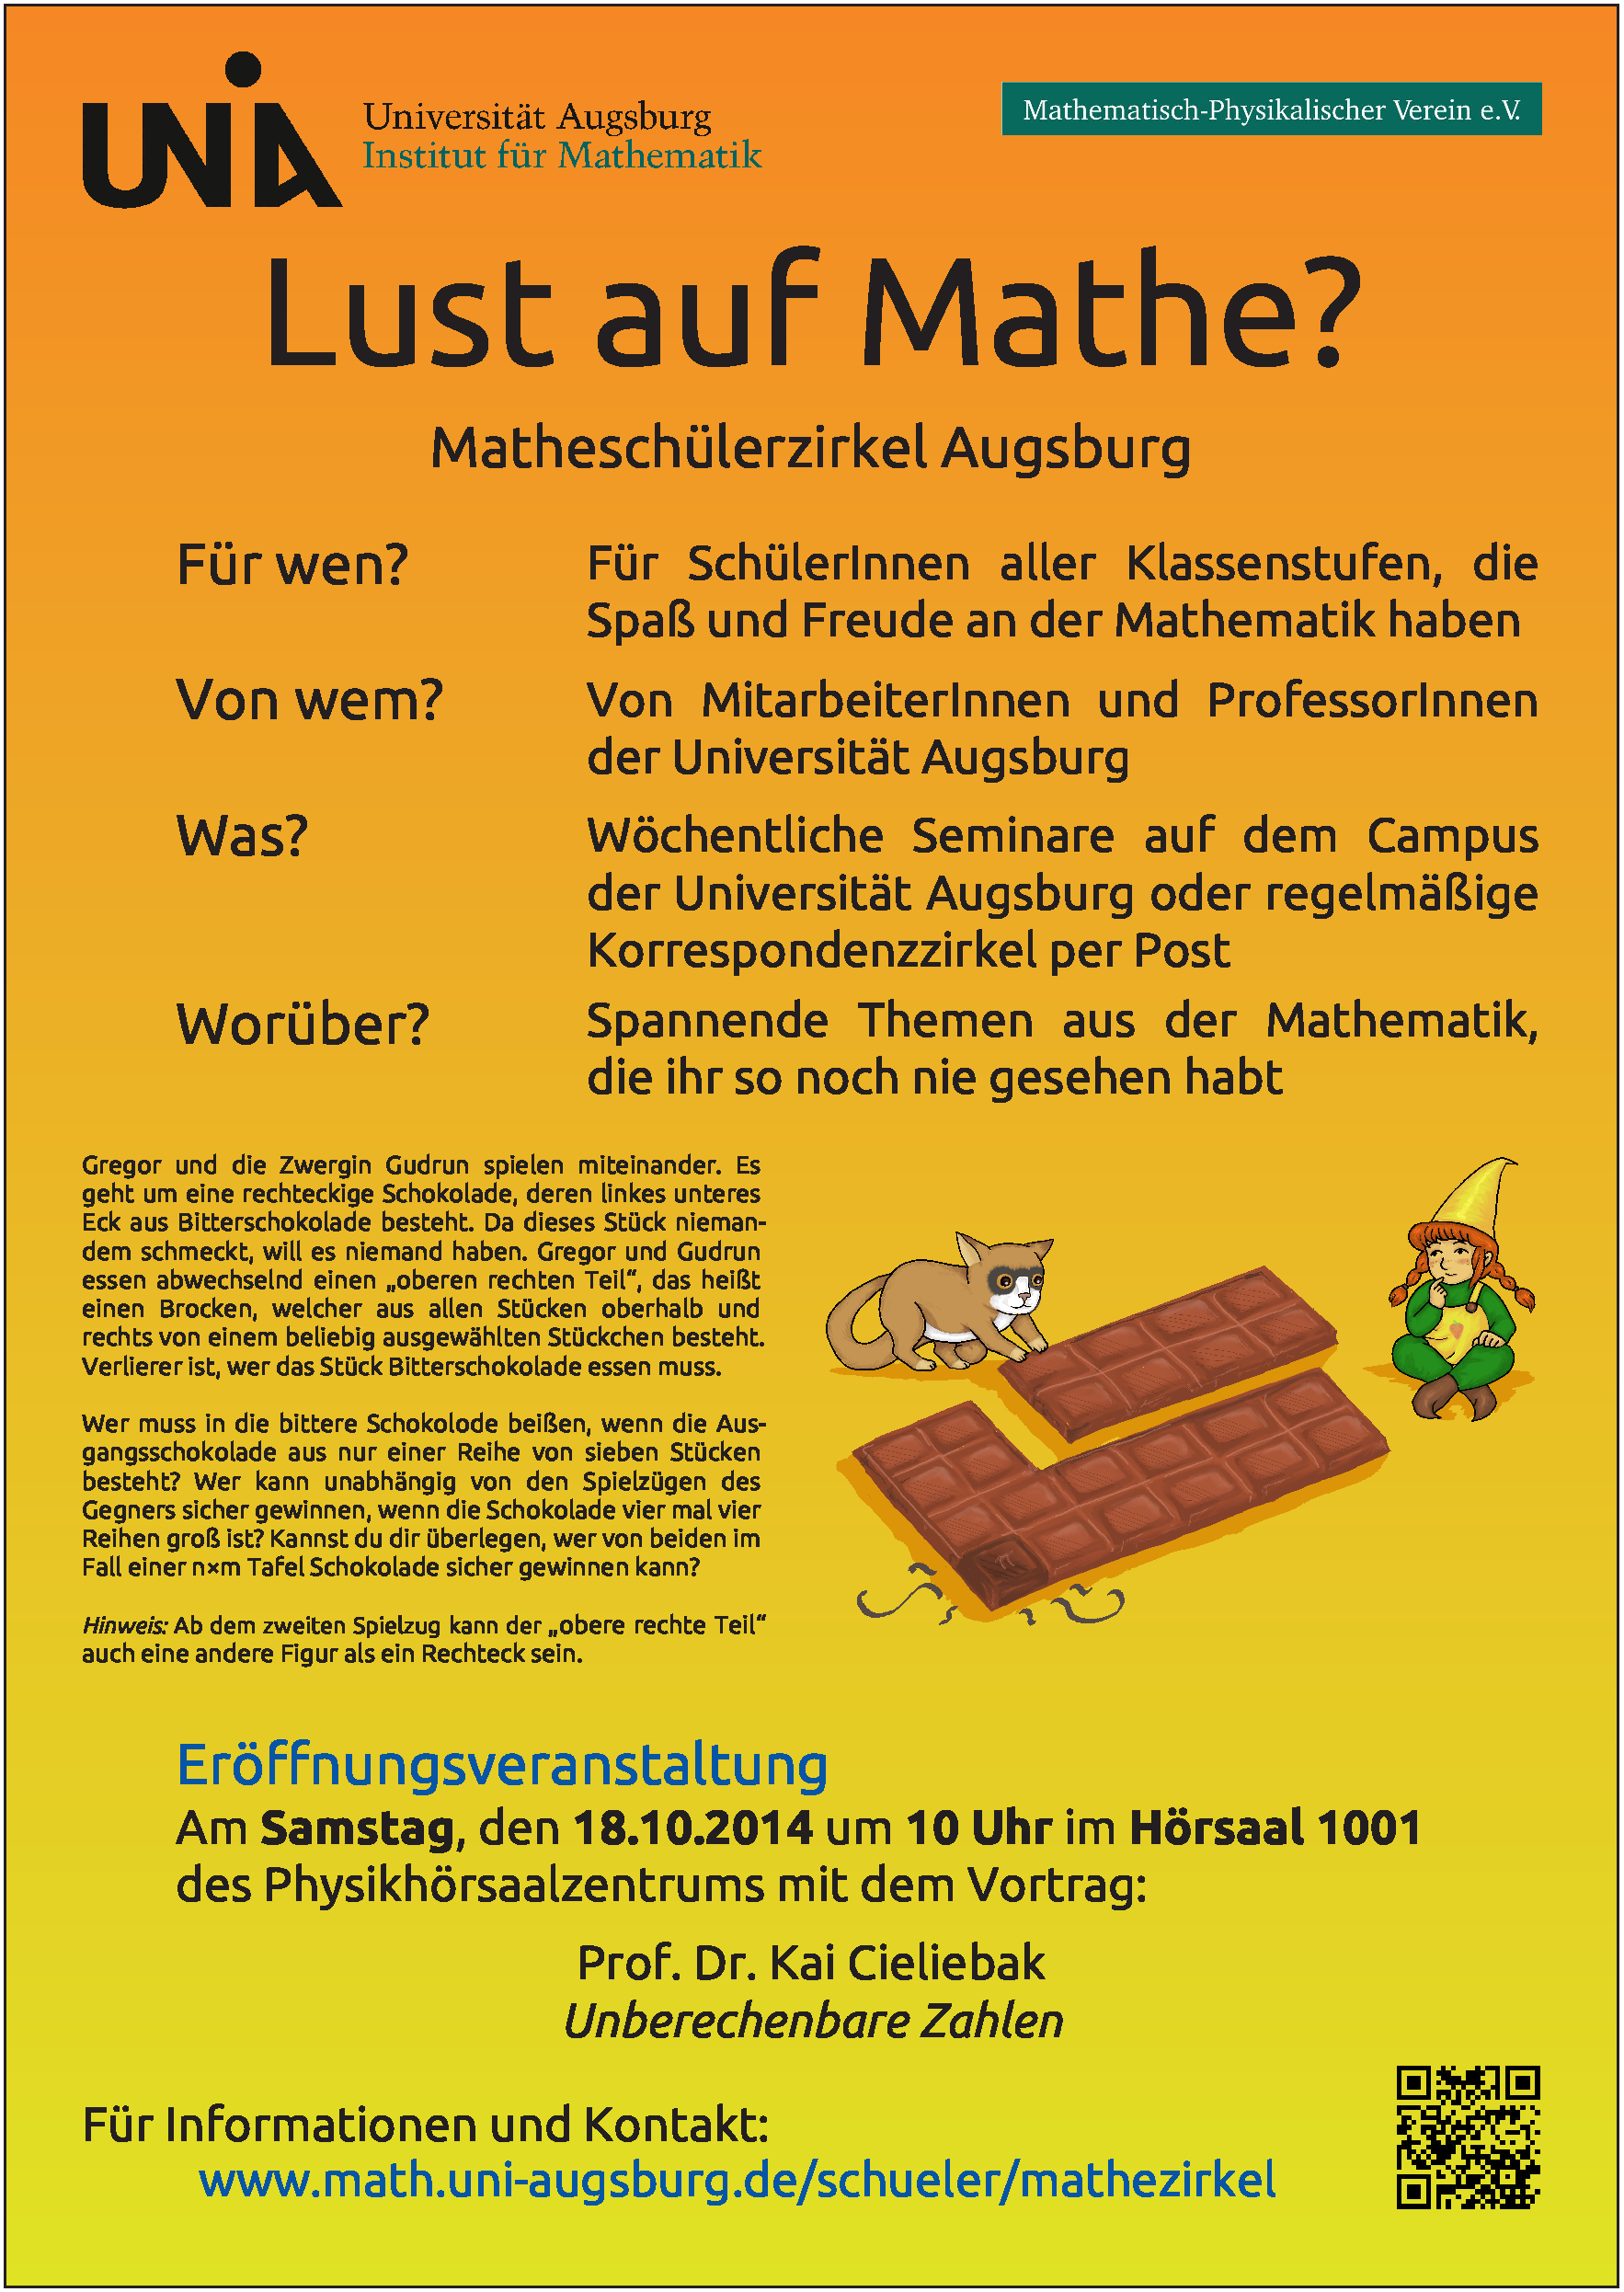
\includegraphics[height=\paperheight]{images/plakat}
    \par
    \transduration{5}\transfade[duration=0.3]
  \end{frame}
}
\imgslidetrans{images/auftakt1}
\imgslidetrans{images/auftakt2}
\imgslidetrans{images/auftakt3}
\imgslidetrans{images/auftakt3-beschriftet}
\imgslidetrans{images/auftakt4}

\imgslidetrans{images/mathecamp01}
\imgslidetrans{images/mathecamp02}
\imgslidetrans{images/mathecamp03}
\imgslidetrans{images/mathecamp04}
\imgslidetrans{images/mathecamp11}
\imgslidetrans{images/mathecamp05}
\imgslidetrans{images/mathecamp06}
\imgslidetrans{images/mathecamp07}
\imgslidetrans{images/mathecamp08}
\imgslidetrans{images/mathecamp09}
\imgslidetrans{images/mathecamp10}
\imgslidetrans{images/mathecamp12}
\imgslidetrans{images/mathecamp-space}
\imgslidetrans{images/mathecamp-gruppenfoto}

\usebackgroundtemplate{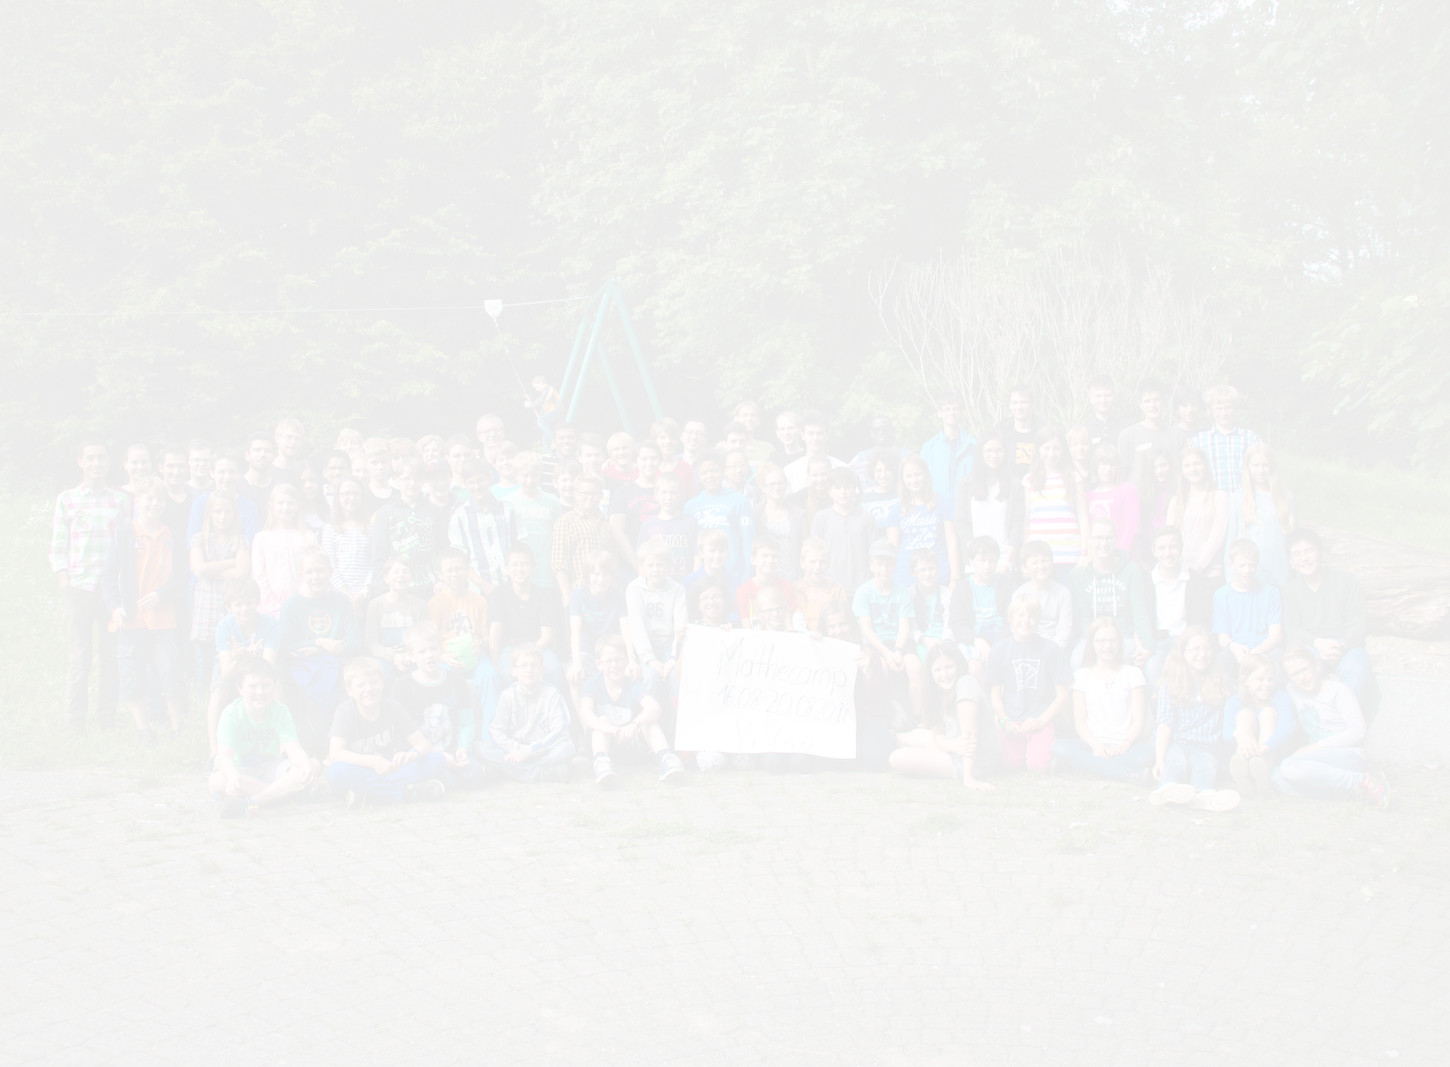
\includegraphics[height=\paperheight]{images/mathecamp-gruppenfoto-desaturiert}}
\begin{frame}
  \centering\large
  \qquad\quad\!\!
\includegraphics[width=0.3\textwidth]{images/gregor}
  \bigskip

  An SchülerInnen, Eltern und LehrerInnen: \\
  \hil{Mathecamp vom 20. bis 26. August}
  \bigskip

  An StudentInnen und DoktorandInnen: \\
  \hil{Gründet ebenfalls solche Zirkel!}
  \par
\end{frame}

\end{document}
